\section{Group lasso}
\citep{group_lasso} introducerede en generalisering af standard lasso kaldet group lasso, som tillader at forudbestemte grupper af prædiktorer vælges eller fravælges, således at alle prædiktorer i en specifik gruppe er enten inkluderet eller ikke inkluderet.
%Group lasso tillader grupper af relateret prædiktorer at blive valgt som en enkelt enhed, som kan bruges i situationer, hvor det ikke giver mening af at inkludere nogle prædiktorer og ikke andre.
Afsnittet er skrevet udfra kapitel 4 i \citep{hastie} samt \citep{group_lasso}.
%I mange regressions problemer har prædiktorerne en naturlig grupperet struktur, og da foretrækkes det at alle koefficienter indenfor en gruppe er ikke-nul (eller nul) samtidig.

Betragt en lineær regressions model med $J$ grupper af prædiktorer, hvor vektoren $\mathbf{Z}_j \in \R^{p_j}$ repræsenterer prædiktorerne i gruppe $j$ for $j=1, \ldots, J$.
Formålet er da, at prædiktere responsvariablen $y \in \R$ baseret på en samling af prædiktorer $(\mathbf{Z}_1,\ldots, \mathbf{Z}_J)$.
%En lineær model for regressions funktionen $\E{Y \vert Z}$ er givet ved \(\theta_0 + \sum_{j=1}^J Z_j^T \theta_j\), hvor $\theta_j \in \R^{p_j}$ repræsenterer en gruppe af $p_j$ regressions koefficienter. 

Givet \(n\) observationer \(\cbr{ \del{y_i, z_{i,1}, z_{i,2}, \ldots, z_{i,J}}}_{i=1}^n\) løser group lasso følgende optimeringsproblem
\begin{align}
\hat{\beta}_j^{\text{group lasso}} = \argmin_{\ttheta_j \in \R^{p_j}} \cbr{\frac{1}{2} \sum_{i=1}^n \del{y_i - \sum_{j=1}^J z_{ij}^T \ttheta_j}^2 + \lambda \sum_{j=1}^J \Vert \ttheta_j \Vert_2}. \label{eq:4.5}
\end{align}
Dette er en grupperet generalisering af lasso, som har følgende egenskaber:
\begin{itemize}
\item Afhængig af $\lambda$, vil enten alle indgange i vektoren $\hat{\ttheta}_j$ være nul eller ikke-nul
\item Når $p_j=1$, da har vi at $\Vert \ttheta_j \Vert_2 = \vert \ttheta_j \vert$, således at alle grupper er singletons, dermed reduceres optimeringsproblemet \eqref{eq:4.5} til standard lasso.
\end{itemize}
Figur \ref{fig:group_lasso} viser betingelsesområderne for henholdsvis group lasso og standard lasso for tre variable.
%Vi ser at den grupperet lasso deler egenskaber med både $\ell_1$ og $\ell_2$ kuglen.
%
\begin{figure}[H]
\centering
 \scalebox{0.5}{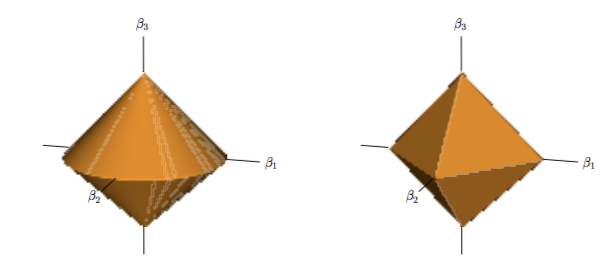
\includegraphics{fig/group_lasso.jpg}}
\caption{Til venstre ses kuglen for group lasso i \(\R^3\) og til højre ses \(\ell_1\) kuglen.
I dette tilfælde har vi to grupper med koefficienter \(\ttheta_1 = \del{\beta_1, \beta_2} \in \R^2\) og \(\theta_2 = \beta_3 \in \R\).}
\label{fig:group_lasso}
\end{figure}
%
I \eqref{eq:4.5} straffes alle grupper ligeligt, hvilket betyder at større grupper vil have en tendens til at blive valgt.
\citep{group_lasso} anbefalede at vægte strafleddene for hver gruppe i forhold til gruppens størrelse med en factor \(\sqrt{p_j}\).

\subsection{Udregning af group lasso}

Lad os omskrive optimeringsproblemet \eqref{eq:4.5} på matrix-vektor form
\begin{align}
\hat{\tbeta}^{\text{group lasso}} = \argmin_{\ttheta_1, \ldots, \ttheta_J} \cbr{\frac{1}{2} \Vert \y - \sum_{j=1}^J \mathbf{Z}_{j} \ttheta_j \Vert_2^2 + \lambda \sum_{j=1}^J \Vert \ttheta_j \Vert_2}. \label{eq:4.11}
\end{align}
For dette problem er nul subgradient ligningerne givet ved
\begin{align*}
- \mathbf{Z}_{j}^T \del{\y - \sum_{\ell=1}^J \mathbf{Z}_\ell \hat{\ttheta}_\ell} + \lambda \hat{\ts}_j = 0, \quad j=1,\ldots, J,
\end{align*} 
hvor $\hat{\ts}_j \in \R^{p_j}$ er et element af subdifferentialet af normen $\Vert \cdot \Vert_2$ evalueret i $\hat{\ttheta}_j$.
Når $\hat{\ttheta}_j \neq 0$, har vi, at $\hat{\ts}_j = \frac{\hat{\ttheta}_j}{\Vert \hat{\ttheta}_j \Vert_2}$, og når $\hat{\ttheta}_j=0$, har vi, at $\hat{\ts}_j$ er enhver vektor hvor $\Vert \hat{\ts}_j \Vert_2 \leq 1$.
En metode til at løse nul subgradient ligningerne er ved at fastholde alle block vektorer $\cbr{\hat{\ttheta}_k, k \neq j}$, og da løse for $\hat{\ttheta}_j$.
Hermed udføres block coordinate descent på objektfunktionen af group lasso.
Da problemet er konveks, og strafleddet kan separeres efter block, er det garanteret at konvergere til en optimal løsning.

Med $\cbr{\hat{\ttheta}_k, k \neq j}$ fastholdt, kan vi skrive
\begin{align*}
- \mathbf{Z}_{j}^T \del{\mathbf{r}_j - \mathbf{Z}_j \hat{\ttheta}_j} + \lambda \hat{\ts}_j = 0,
\end{align*}
hvor $\mathbf{r}_j = \y - \sum_{k \neq j} \mathbf{Z}_k \hat{\ttheta}_k $ er j'te partial residual.
Fra betingelserne opfyldt af subgradienten $\hat{\ts}_j$, må vi have at $\hat{\ttheta}_j =0$ hvis $\Vert \mathbf{Z}_j^T \mathbf{r}_j \Vert_2 < \lambda$, og ellers må $\hat{\ttheta}_j$ opfylde
\begin{align}
\hat{\ttheta}_j = \del{\mathbf{Z}_j^T \mathbf{Z}_j + \frac{\lambda}{\Vert \hat{\ttheta}_j \Vert_2} \mathbf{I}}^{-1} \mathbf{Z}_j^T \mathbf{r}_j. \label{eq:4.14}
\end{align}
Denne opdatering minder om løsningen af ridge regression, bortset fra at den underliggende strafparameter afhænger af $\Vert \hat{\ttheta}_j \Vert_2$.
Ligning \eqref{eq:4.14} har desværre ikke en lukket løsning for $\hat{\ttheta}_j$, medmindre at $\mathbf{Z}_j$ er ortonormal. 
I dette special tilfælde har vi, at
\begin{align*}
\hat{\ttheta}_j = \del{1 - \frac{\lambda}{\Vert \mathbf{Z}_j^T \mathbf{r}_j \Vert_2}}_+  \mathbf{Z}_j^T \mathbf{r}_j.
\end{align*}
Algoritmen er stabil og vil normal nå en fornuftig konvergens tolerance indenfor få iterationer.
De computermæssig byrde vil stige voldsomt når antallet af prædiktorer stiger.


Nedenfor beskrives kort nogle udvidelser af group lasso nemlig sparse group lasso samt overlap group lasso.
%
\subsection{Sparse group lasso}
Sparse group lasso udfører variabeludvælgelse indenfor de valgte grupper, hvorimod group lasso blot udvælger grupperne.
For at opnå denne sparsity indenfor grupperne tilføjes en \(\ell_1\) norm til standard group lasso \eqref{eq:4.11} 
\begin{align*}
\argmin_{\cbr{\ttheta_j \in \R^{p_j}}_j=1^J} \cbr{\frac{1}{2} \Vert \y - \sum_{j=1}^J \mathbf{Z}_{j} \ttheta_j \Vert_2^2 + \lambda \sum_{j=1}^J \sbr{ \del{1-\alpha} \Vert \ttheta_j \Vert_2 + \alpha \Vert \ttheta_j \Vert_1}},
\end{align*}
hvor \(\alpha \in \sbr{0,1}\).
For \(\alpha = 0 \) fås group lasso og for \(\alpha = 1\) fås standard lasso.

Figur \ref{fig:sparse_group_lasso} viser betingelsesområderne for henholdsvis group lasso og sparse group lasso for tre variable.
Bemærk at for de to horisontale akser, da ligner betingelsesområdet det for elastisk net.
%
\begin{figure}[H]
\centering
 \scalebox{0.5}{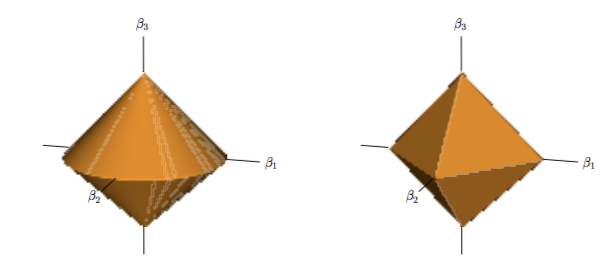
\includegraphics{fig/group_lasso.jpg}}
\caption{Til venstre ses kuglen for group lasso i \(\R^3\) og til højre sparse group lasso kuglen med \(\alpha = 0.5\).
Igen har vi to grupper med koefficienter \(\ttheta_1 = \del{\beta_1, \beta_2} \in \R^2\) og \(\theta_2 = \beta_3 \in \R\).}
\label{fig:group_lasso}
\end{figure}
%



udvide group lasso til sparse group lasso, som kan vælge individuelle kovaraiter indenfor en gruppe, ved at tilføje en ekstra \(\ell_1\) penalty to hver gruppe underrum.


\subsection{Overlap group lasso}
En anden udvidelse af group lasso tillader overlap mellem grupperne, dvs at prædiktorerne kan tilhører mere end én gruppe.

\newpage